\section{The Geometry of High-Dimensional Representation Spaces}
\label{sec:geometry}

The utility of any vectorial representation ultimately depends on how efficiently the encoder exploits the available capacity of $\mathbb{R}^d$. A representation-space in which all vectors collapse into a narrow cone wastes capacity and a space in which a few points dominate the neighbourhood structure is structurally unstable. These qualities can be diagnosed purely from the intrinsic geometry of $\mathcal{Z}$, before any downstream task is even defined \cite{ethayarajh-2019-contextual, GaoHTQWL19}. 

That geometric regularity limits representational quality was recognised early across paradigms. Implicitly by \citet{Salton_AVS_1975} through angular discriminability in the term-document space, by \citet{Deerwester_1990_Indexing} through the low effective rank revealed by \acs{SVD} and by \citet{Mikolov2013} through the presupposition that vector arithmetic carries semantic meaning. While originally articulated for frequency-based and static representations, these desiderata prove equally critical for modern contextual encoders, where recent studies demonstrate that Transformer-based embeddings also suffer from geometric pathologies \citep{mu2018allbutthetop, ethayarajh-2019-contextual, bis_too_2021}. 

%(Bi´ s et al., 2021; Mickus et al., 2019; Ethayarajh, 2019; Coenen et al., 2019b; Cai et al., 2021; Mu et al., 2017; Liang et al., 2021).


% ================================================================
% 2.2.1  ISOTROPY
% ================================================================
\subsection{Global Distributional Regularity: Isotropy}
\label{sec:isotropy}

One of the most essential properties of a well-structured embedding space is that it should be isotropic, meaning that the variance of the representations is distributed uniformly across all available dimensions.  If variance is evenly distributed, no single spatial direction disproportionately dominates similarity computations, enabling the space to achieve maximum dynamic range to discriminate between nuanced semantic concepts \cite{rudman-etal-2022-isoscore, Cai2021IsotropyIT}.

\begin{definition}[Isotropy]
\label{def:isotropy}
A set of embeddings $\{\mathbf{z}_1, \dots, \mathbf{z}_N\} \in \mathcal{Z} \subset \mathbb{R}^d$ with centroid $\boldsymbol{\mu} = \frac{1}{N}\sum_{i=1}^N \mathbf{z}_i$ is called \emph{isotropic} if its covariance matrix $\boldsymbol{\Sigma}$ is proportional to the identity matrix $\mathbf{I}_d$:
\begin{equation}
    \boldsymbol{\Sigma} 
    = \frac{1}{N}\sum_{i=1}^{N} (\mathbf{z}_i - \boldsymbol{\mu}) (\mathbf{z}_i - \boldsymbol{\mu})^\top 
    = \sigma^2 \mathbf{I}_d
    \label{eq:cov_matrix}
\end{equation}
The eigendecomposition $\boldsymbol{\Sigma} = \mathbf{Q}\,\mathrm{diag}(\lambda_1, \dots, \lambda_d)\,\mathbf{Q}^\top$ of a perfectly isotropic space yields identical eigenvalues $\lambda_1 = \dots = \lambda_d = \sigma^2$. 
Consequently, the expected cosine similarity between two randomly drawn vectors converges to zero as $d \to \infty$ \cite[]{rudman-etal-2022-isoscore, Cai2021IsotropyIT}.
\end{definition}

In practice, however, contextual representations are frequently highly anisotropic. They tend to cluster within a narrow cone in $\mathbb{R}^d$, leaving most of the space unused \cite{ethayarajh-2019-contextual, GaoHTQWL19}.  To understand the consequences of this degeneration, any embedding can be decomposed into the global corpus centroid and a specific semantic residual component, $\mathbf{z}_i = \boldsymbol{\mu} + \tilde{\mathbf{z}}_i$. For $L_2$-normalised vectors, the inner product then expands as

\begin{equation}
    \mathbf{z}_i^\top \mathbf{z}_j 
    = \underbrace{\|\boldsymbol{\mu}\|_2^2}_{\text{constant bias}}
    + \underbrace{\boldsymbol{\mu}^\top \tilde{\mathbf{z}}_j 
    + \tilde{\mathbf{z}}_i^\top \boldsymbol{\mu}}_{\text{mean--residual interaction}}
    + \underbrace{\tilde{\mathbf{z}}_i^\top \tilde{\mathbf{z}}_j}_{\text{semantic signal}} .
    \label{eq:mean_shift}
\end{equation}

The term $\|\boldsymbol{\mu}\|_2^2$ acts as a constant bias for all vector pairs. When this term is large relative to the actual semantic residual $\tilde{\mathbf{z}}_i^\top \tilde{\mathbf{z}}_j$, it overshadows every comparison, so that, all vectors appear artificially similar to one another\footnote{In a theoretical setting with perfect numerical precision, this constant bias would not affect the downstream ranking, as adding a constant to all similarities preserves their relative order. In practice, however, modern hardware relies on limited floating-point arithmetic. When the semantic variance is infinitesimally small compared to the massively dominant constant bias, it is frequently lost to rounding errors, effectively destroying the retrieval signal \cite{GaoHTQWL19}.} \cite{ethayarajh-2019-contextual,mu2018allbutthetop}. 

\begin{figure}[htpb]
    \centering
    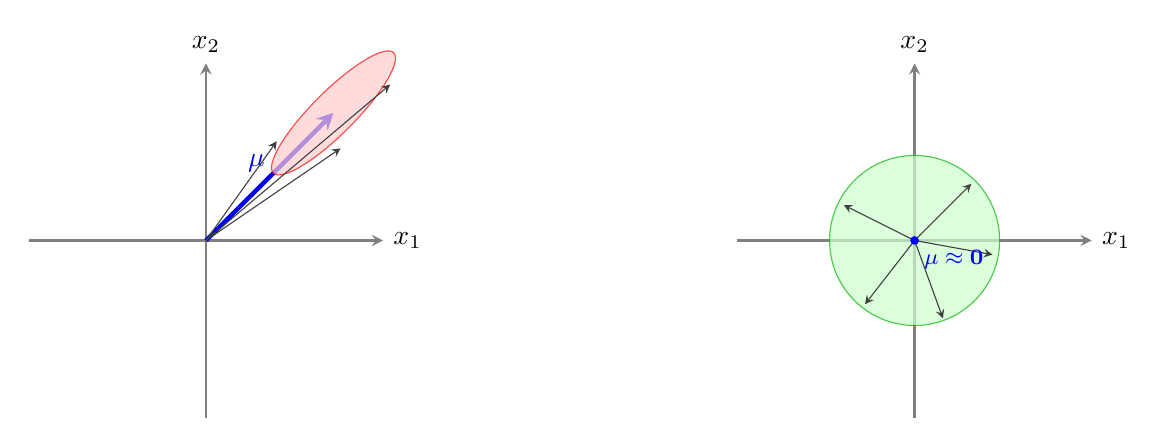
\begin{tikzpicture}[>=stealth, scale=0.9, font=\sffamily]

        % Define constants for symmetry
        \def\axislen{2.5}

        % --- Left Panel: Anisotropic (Mean-Shifted) ---
        \begin{scope}[xshift=-5cm] % Position the left diagram
            % Symmetrical Axes
            \draw[->, thick, gray] (-\axislen, 0) -- (\axislen, 0) node[right, text=black] {$x_1$};
            \draw[->, thick, gray] (0, -\axislen) -- (0, \axislen) node[above, text=black] {$x_2$};

            % Mean vector showing the shift (ultra thick blue)
            \coordinate (mu) at (1.8, 1.8);
            \draw[->, ultra thick, blue] (0,0) -- (mu) node[midway, above left, text=blue, inner sep=1pt] {$\boldsymbol{\mu}$};

            % Anisotropic Distribution (ellipse) far from origin
            \draw[fill=red!20, draw=red, opacity=0.7, rotate around={45:(mu)}] (mu) ellipse (1.2cm and 0.3cm);

            % Sample vectors (all starting from origin) forming a cone
            \draw[->, thin, darkgray] (0,0) -- (2.6, 2.2);
            \draw[->, thin, darkgray] (0,0) -- (1.0, 1.4);
            \draw[->, thin, darkgray] (0,0) -- (1.9, 1.3);

        \end{scope}

        % --- Right Panel: Isotropic ---
        \begin{scope}[xshift=5cm] % Position the right diagram
            % Symmetrical Axes (same size as left)
            \draw[->, thick, gray] (-\axislen, 0) -- (\axislen, 0) node[right, text=black] {$x_1$};
            \draw[->, thick, gray] (0, -\axislen) -- (0, \axislen) node[above, text=black] {$x_2$};

            % Isotropic Distribution (circle) centered at origin
            \draw[fill=green!20, draw=green!70!black, opacity=0.7] (0,0) circle (1.2cm);

            % Sample vectors (pointing everywhere) starting from origin
            \draw[->, thin, darkgray] (0,0) -- (0.8, 0.8);
            \draw[->, thin, darkgray] (0,0) -- (-1.0, 0.5);
            \draw[->, thin, darkgray] (0,0) -- (0.4, -1.1);
            \draw[->, thin, darkgray] (0,0) -- (-0.7, -0.9);
            \draw[->, thin, darkgray] (0,0) -- (1.1, -0.2);

            % Mean Vector at Origin is zero (small blue point)
            \filldraw[blue] (0,0) circle (1.5pt) node[below right, text=blue, font=\footnotesize] {$\boldsymbol{\mu} \approx \mathbf{0}$};

        \end{scope}

    \end{tikzpicture}
    \caption[Visual comparison of representation space geometry.]{Visual comparison of representation space geometry. \textbf{Left:} A pathological, anisotropic space, where embeddings form a narrow cone shifted away from the origin. \textbf{Right:} An ideal, isotropic space where the full dynamic range of $\mathbb{R}^d$ is utilized for semantic discrimination, with a centered centroid. (Own illustration)}
    \label{fig:isotropy_comparison}
\end{figure}


To systematically assess the extent of this geometric degeneration, visualized in Figure~\ref{fig:isotropy_comparison}, several metrics have been proposed. The most direct and intuitive symptom is a high baseline angular similarity between random representations \cite{ethayarajh-2019-contextual, rudman-etal-2022-isoscore, wang-isola-2020-contrastive,roy2007effective}.

\begin{metricbox}[Metric: Average Pairwise Cosine Similarity $\bar{s}_{\cos}$ \cite{ethayarajh-2019-contextual}]
\begin{equation}
    \bar{s}_{\cos} = \mathbb{E}_{i \neq j}[\cos(\mathbf{z}_i, \mathbf{z}_j)] = \binom{N}{2}^{\!-1} \sum_{i < j} \frac{\mathbf{z}_i^\top \mathbf{z}_j}{\|\mathbf{z}_i\|_2\;\|\mathbf{z}_j\|_2}
    \label{met:avg_cosine}
\end{equation}
\textbf{Ideal:} $\approx 0$ (diverse directions) \quad \textbf{Pathological:} $\to 1$ (cone-shaped concentration)
\end{metricbox}

Isolating the primary cause of this baseline similarity compression requires examining the global centroid of the representations \cite{yamagiwa2025norm}. \citet{mu2018allbutthetop} and \citet{ethayarajh-2019-contextual} originally demonstrated that contextual embeddings share a massively dominant common vector. Building upon these observations, \citet{yamagiwa2025norm} formalized the phenomenon by mathematically decomposing the mean squared norm of contextualized embeddings into their true semantic variance and the squared norm of their mean embedding. Following their framework, the exact influence of this spatial shift can be strictly quantified by the mean dominance ratio $D_\mu$, which measures the proportion of the vector magnitude that is merely a shared spatial artifact rather than unique semantic information.


\begin{metricbox}[Metric: Mean Dominance Ratio $D_\mu$ \cite{yamagiwa2025norm}]
\begin{equation}
    D_\mu = \frac{\|\boldsymbol{\mu}\|_2^2}{\frac{1}{N}\sum_{i=1}^N \|\mathbf{z}_i\|_2^2}
    \label{met:mean_dominance_ratio}
\end{equation}
\textbf{Ideal:} $0$ (centroid at origin) \quad \textbf{Pathological:} $\to 1$ (constant bias dominates)
\end{metricbox}

While $D_\mu$ captures the translational shift away from the origin, it does not describe the shape of the variance. Moving beyond simple mean-shifts, the eigenvalue spectrum of the covariance matrix provides a comprehensive view of how the remaining variance is distributed and IsoScore quantifies how uniformly this variance is distributed across the embedding dimensions \cite{rudman-etal-2022-isoscore}.

\begin{metricbox}[Metric: IsoScore \citep{rudman-etal-2022-isoscore}]
Let $\lambda_1 \geq \dots \geq \lambda_d$ be the eigenvalues of $\boldsymbol{\Sigma}$ and $\bar{\lambda}$ their mean. 
\begin{equation}
    \text{IsoScore} = 1 - \frac{d \sum_{i=1}^d (\lambda_i - \bar{\lambda})^2}{(d-1)\left(\sum_{i=1}^d \lambda_i\right)^2}
    \label{met:isoscore}
\end{equation}
\textbf{Ideal:} $1$ (all eigenvalues equal) \quad \textbf{Pathological:} $\to 0$ (single dominant direction)
\end{metricbox}

An alternative, non-spectral approach probes the spatial density of the embedding space by evaluating its response to arbitrary directional unit vectors. This partition function evaluates whether the embeddings densely populate all directions or cluster along a few specific axes \cite{Arora2016_Latent, mu2018allbutthetop}.

\begin{metricbox}[Metric: Partition Function Isotropy $I_{\mathrm{PF}}$ \cite{Arora2016_Latent, mu2018allbutthetop}]
For a random unit vector $\mathbf{c} \in \mathbb{S}^{d-1}$, define the partition function $Z(\mathbf{c}) = \frac{1}{N}\sum_{j=1}^{N} \exp(\mathbf{z}_j^\top \mathbf{c})$. Isotropy is then defined as the ratio of the minimum to the maximum response:
\begin{equation}
    I_{\mathrm{PF}} = \frac{\min_{\mathbf{c}}\; Z(\mathbf{c})}{\max_{\mathbf{c}}\; Z(\mathbf{c})}
    \label{met:partition_function_isotropy}
\end{equation}
\textbf{Ideal:} $1$ ($Z$ constant across all directions) \quad \textbf{Pathological:} $\to 0$ (strong directional dependence)
\end{metricbox}

Finally, the simplest spectral diagnostic bounds the variance imbalance by comparing the extreme ends of the eigenvalue spectrum. This condition number serves as a direct indicator of how strongly the variance collapses into the first few principal components \cite{rudman-etal-2022-isoscore,ethayarajh-2019-contextual}\cite[p.~88~f.]{golub2013matrix}.

\begin{metricbox}[Metric: Eigenvalue Ratio $R_\lambda$ \cite{rudman-etal-2022-isoscore,ethayarajh-2019-contextual}]
The condition number of the covariance matrix, expressed as the ratio of its largest to smallest eigenvalue:
\begin{equation}
    R_\lambda = \frac{\lambda_1}{\lambda_d}
    \label{met:eigenvalue_ratio}
\end{equation} 
\textbf{Ideal:} $1$. \quad \textbf{Pathological:} $\gg 1$ (variance concentration along the first \acp{PC}).
\end{metricbox}



% ================================================================
% 2.2.2  INTRINSIC DIMENSIONALITY
% ================================================================
\subsection{Information Density and Intrinsic Dimensionality}
\label{sec:intrinsic_dim}

Although embeddings reside in a high-dimensional space $\mathbb{R}^d$ e.g., $d=768$ or $d=3072$, the actual data typically concentrate on a manifold of significantly lower dimensionality \cite{Fefferman2016_Manifold}. The intrinsic dimensionality $d_{\mathrm{int}}$ measures the minimum number of degrees of freedom required to capture the meaningful semantic variance of the dataset, treating the remaining dimensions as negligible statistical noise \cite{AnsuiniLLZ19}. If $d_{\mathrm{int}}$ remains high relative to the ambient dimension $d$, the representation space uses its capacity efficiently. Conversely, a very low relative intrinsic dimension indicates a highly redundant encoding where semantic nuance is compressed into a few dominant components. To operationalise this manifold concept for empirical evaluation, global spectral estimators quantify this effective dimensionality continuously through the eigenvalue spectrum of the covariance matrix \cite{AnsuiniLLZ19, Gao2017Multineuronal}. A measure of the effective rank that represents the number of equally contributing dimensions is the \ac{PR} \cite{Gao2017Multineuronal}.

\begin{metricbox}[Metric: Participation Ratio (\acs{PR}) \cite{Gao2017Multineuronal}]
\begin{equation}
    \mathrm{\ac{PR}} = \frac{\left(\sum_{i=1}^d \lambda_i\right)^2}{\sum_{i=1}^d \lambda_i^2}
    \label{met:participation_ratio}
\end{equation}
\textbf{Ideal:} $\mathrm{\ac{PR}} \approx d$ (perfect isotropy) \quad \textbf{Pathological:} $\mathrm{\ac{PR}} \to 1$ (variance collapses into a single dimension)
\end{metricbox}


While \ac{PR} uses the sum of the squares of the eigenvalues, the effective rank is based on the Shannon entropy of the eigenvalue distribution. It provides a more precise measure of how many dimensions effectively carry information \cite{roy2007effective}.

\begin{metricbox}[Metric: Effective Rank \citep{roy2007effective}]
Let $p_i = \lambda_i / \sum_{j=1}^d \lambda_j$ be the normalized eigenvalues, forming a probability distribution. The effective rank is the exponential of the Shannon entropy $H$:
\begin{equation}
    \text{Effective Rank} = \exp\left( -\sum_{i=1}^d p_i \ln p_i \right)
    \label{met:effective_rank}
\end{equation}
\textbf{Ideal:} $\approx d$ (uniform variance distribution) \quad \textbf{Pathological:} $1$ (all variance in one dimension)
\end{metricbox}

For a more discrete threshold, the cumulative explained variance determines the minimal subspace dimensionality capturing the majority of the signal \cite{Gao2017Multineuronal}\cite[p. 325 f.]{deisenroth2020mathematics}. 

\begin{metricbox}[Metric: \acs{PCA} Explained Variance Threshold $d_\alpha$ \citep{Gao2017Multineuronal,deisenroth2020mathematics}]
The smallest number of principal components $k$ required to explain a fixed threshold $\alpha$ of the total variance:
\begin{equation}
    d_\alpha = \min \left\{ k \;\middle|\; \frac{\sum_{i=1}^k \lambda_i}{\sum_{i=1}^d \lambda_i} \geq \alpha \right\}
    \label{met:pca_explained_variance}
\end{equation}
\textbf{Ideal:} High $d_\alpha$ relative to $d$ \quad \textbf{Pathological:} $d_\alpha \ll d$
\end{metricbox}


While spectral methods capture global structure, they may miss locally varying dimensionality. Local estimators instead exploit the scaling behaviour of Euclidean distances in the immediate neighbourhood of each point \cite{Levina2004_MLE}.

\begin{metricbox}[Metric: Maximum Likelihood Estimator (MLE) \citep{Levina2004_MLE}]
For a point $\mathbf{z}$ with $k$-nearest-neighbour distances $r_1 \leq \dots \leq r_k$, the local topological dimension is estimated as:
\begin{equation}
    \hat{d}_{\mathrm{MLE}}(\mathbf{z}) = \left[ \frac{1}{k-1}\sum_{j=1}^{k-1} \log\frac{r_k}{r_j} \right]^{-1}
    \label{met:MLE}
\end{equation}
The corpus-level estimate is obtained by averaging over all points. \\
\textbf{Ideal:} High $\hat{d}_{\mathrm{MLE}}$ \quad \textbf{Pathological:} $\hat{d}_{\mathrm{MLE}} \to 1$
\end{metricbox}

MLE is often sensitive to fluctuations in density. The \ac{TwoNN} estimator offers a more robust local alternative by considering only the ratio of distances to the first and second nearest neighbors, which makes it invariant to local differences in density \cite{facco_estimating_2017}.

\begin{metricbox}[Metric: \ac{TwoNN} Estimator \citep{facco_estimating_2017}]
Let $r_1$ and $r_2$ be the distances to the first and second nearest neighbors. The distance ratio is defined as $\mu = r_2 / r_1 \geq 1$. In a space of intrinsic dimension $d$, the cumulative distribution function of $\mu$ is $F(\mu) = 1 - \mu^{-d}$. The intrinsic dimension is estimated by finding the slope $d$ of the linear relationship:
\begin{equation}
    \log(1 - F(\mu)) = -d \log(\mu)
    \label{met:twonn}
\end{equation}
\textbf{Ideal:} High $d$ relative to ambient space \quad \textbf{Pathological:} $d \to 1$
\end{metricbox}


% ================================================================
% 2.2.3  ALIGNMENT AND UNIFORMITY
% ================================================================
\subsection{Local Topology: Alignment and Uniformity}
\label{sec:alignment_uniformity}

\citet{wang-isola-2020-contrastive} decompose the quality of representations on the unit hypersphere $\mathbb{S}^{d-1}$ into two converse properties. These form the theoretical foundation of modern Contrastive Learning frameworks such as SimCSE, which explicitly optimise the InfoNCE loss to simultaneously maximise alignment and uniformity \cite{gao-etal-2021-simcse}. When ground-truth semantic relationships are known, alignment measures how robustly the encoder maps related inputs to adjacent points \cite{wang-isola-2020-contrastive}.

\begin{metricbox}[Metric: Alignment \citep{wang-isola-2020-contrastive}]
Given a distribution of semantically related (positive) pairs $p_{\mathrm{pos}}$, alignment is defined as the expected distance between them:
\begin{equation}
    \mathcal{L}_{\mathrm{align}} = \mathbb{E}_{(x,\, x^+) \sim p_{\mathrm{pos}}} \bigl[\|\phi_\theta(x) - \phi_\theta(x^+)\|_2^2\bigr]
    \label{met:alignment}
\end{equation}
\textbf{Ideal:} Low $\mathcal{L}_{\mathrm{align}}$ (positive pairs are mapped closely) \quad \textbf{Pathological:} High $\mathcal{L}_{\mathrm{align}}$
\end{metricbox}

Opposite to alignment, uniformity evaluates the overall spatial distribution of the representations without requiring labelled pairs. A perfectly isotropic representation projected onto $\mathbb{S}^{d-1}$ achieves high uniformity \cite{wang-isola-2020-contrastive}.

\begin{metricbox}[Metric: Uniformity \citep{wang-isola-2020-contrastive}]
Uniformity measures how evenly the marginal distribution of all representations covers the hypersphere:
\begin{equation}
    \mathcal{L}_{\mathrm{uniform}} = \log\;\mathbb{E}_{x,\, y \,\sim\, p_{\mathrm{data}}} \bigl[e^{-t\,\|\phi_\theta(x) - \phi_\theta(y)\|_2^2}\bigr], \quad t > 0
    \label{met:uniformity}
\end{equation}
\textbf{Ideal:} Low $\mathcal{L}_{\mathrm{uniform}}$ (vectors are spread evenly) \quad \textbf{Pathological:} High $\mathcal{L}_{\mathrm{uniform}}$ (vectors form degenerate clusters)
\end{metricbox}


% ================================================================
% 2.2.4  HUBNESS
% ================================================================
\subsection{Spatial Fairness: Hubness}
\label{sec:hubness}

The curse of dimensionality introduces distortions into the neighbourhood structure of vector spaces. By the law of large numbers, as the dimension $d \to \infty$, the pairwise Euclidean distance between any two independent and identically distributed vectors converges to a constant \citep[p. 172 f.]{Bishop2024}\citep{Beyer1999_NNMeaningful}. Consequently, the relative contrast between the distance of the nearest $D_{\min}$ and farthest $D_{\max}$ neighbour of any arbitrary reference point vanishes by $ \lim_{d \to \infty} \frac{D_{\max} - D_{\min}}{D_{\min}} = 0 $ \cite{Beyer1999_NNMeaningful}.
A direct consequence of this distance concentration is the emergence of hubness. In finite datasets drawn from such high-dimensional distributions, points situated closer to the global data mean act as \emph{hubs}. They appear as the nearest neighbours to a disproportionately large number of other points. On the other hand, points near the spatial boundary become \emph{anti-hubs} that act as nearest neighbours to no other points. To quantify this structural asymmetry, we analyse the distribution of nearest-neighbour occurrences across the dataset \citep{Radovanovic2010_Hubs,feldbauer2019comprehensive,feldbauer_fast_2018}.

\begin{metricbox}[Metric: Hubness Skewness $S_k$ \citep{Radovanovic2010_Hubs,feldbauer2019comprehensive}]
Let $N_k(i)$ be the number of times vector $\mathbf{z}_i$ appears as a $k$-nearest neighbor of all other points. Hubness is measured by the third standardised moment (skewness) of this distribution:
\begin{equation}
    S_k = \frac{\mathbb{E}\left[(N_k - \mu_{N_k})^3\right]}{\sigma_{N_k}^3}
    \label{met:hubness_skewness}
\end{equation}
\textbf{Ideal:} $S_k \approx 0$ (symmetric, hub-free neighbourhood structure) \quad \textbf{Pathological:} $S_k \gg 1$ (emergence of influential hubs)
\end{metricbox}

Hubness is actively reinforced by low intrinsic dimensionality and anisotropy. This is because the irrelevant dimensions act as noise that inflates distances, pushing all points closer together in the relevant subspace \cite{Radovanovic2010_Hubs, feldbauer2019comprehensive}. While skewness measures the asymmetry of the distribution, the fractions express the problem in terms of absolute ratios.

\begin{metricbox}[Metric: Hub and Anti-Hub Fraction \cite{Radovanovic2010_Hubs,feldbauer2019comprehensive}]
Let $N_k(i)$ be the number of times vector $\mathbf{z}_i$ appears as a $k$-nearest neighbor of all other points. The expected value under perfect spatial uniformity is $\mathbb{E}[N_k] = k$. 
\begin{align}
    f_{\mathrm{antihub}} &= \frac{1}{N} \sum_{i=1}^N \mathbb{I}(N_k(i) = 0) 
    \label{met:antihub_fraction} \\
    f_{\mathrm{hub}} &= \frac{1}{N} \sum_{i=1}^N \mathbb{I}(N_k(i) \geq 2k)
    \label{met:hub_fraction}
\end{align}
where $\mathbb{I}(\cdot)$ is the indicator function and $2k$ serves as a standard empirical threshold for hub emergence \cite{feldbauer2019comprehensive}. \\
\textbf{Ideal:} $0$ (all points are retrieved roughly $k$ times) \quad \textbf{Pathological:} $\to 1$
\end{metricbox}

To capture the global inequality of the $N_k$ distribution in a single number, economists often use the Robin Hood Index, also known as the Hoover Index. This index measures the proportion of \emph{nearest-neighbor slots} that would need to be redistributed from the hubs to the anti-hubs in order to achieve perfect equality \cite{feldbauer_fast_2018}.

\begin{metricbox}[Metric: Robin Hood Index \cite{feldbauer_fast_2018}]
Derived from the Gini coefficient framework, the index computes the maximum vertical distance between the Lorenz curve of the $N_k$ distribution and the line of perfect equality:
\begin{equation}
    \text{RHI} = \frac{1}{2} \frac{\sum_{i=1}^N |N_k(i) - k|}{\sum_{i=1}^N N_k(i)}
    \label{met:robin_hood}
\end{equation}
\textbf{Ideal:} $0$ (perfect equality, $N_k(i) = k$ for all) \quad \textbf{Pathological:} $\to 1$ (maximum inequality)
\end{metricbox}

This list of geometric properties is not exhaustive. For instance, additional topological properties such as local clustering coefficients or manifold curvature could be considered to capture more nuanced spatial pathologies. However, the metrics formalised above are fundamentally sufficient to capture the most critical geometric pathologies that degrade downstream retrieval performance.